\section{The Namespace Dependency Graph}
\label{sec:namespace-graph}

The module-level analysis of \S\ref{sec:import-graph} and the declaration-level analysis of \S\ref{sec:theorem-premise} examine the library at two extreme scales. At the module level, each source file is a single vertex; at the declaration level, every theorem and definition is its own vertex. Between these extremes lies a natural intermediate structure: the \emph{namespace}. In Lean~4, every declaration~$d$ carries a fully qualified name---e.g., \decl{Nat.Prime.dvd\_mul}---whose dot-separated components encode a hierarchical naming convention. By truncating names to different depths, we obtain a continuously parameterized family of dependency graphs that interpolates between the coarse module level and the fine declaration level. This section constructs these graphs and measures how \emph{containment}---the proportion of edges that stay within namespace boundaries---decays as granularity increases.

The $308{,}129$ declarations in \module{Mathlib} span six depth levels. Table~\ref{tab:ns-depth-count} shows how the number of distinct namespaces grows with truncation depth.

\begin{table}[ht]
\centering
\caption{Number of distinct namespaces at each truncation depth~$k$.}
\label{tab:ns-depth-count}
\begin{tabular}{cr}
\toprule
Depth $k$ & $|\mathcal{N}_k|$ \\
\midrule
1          & $3{,}184$ \\
2          & $10{,}097$ \\
3          & $13{,}785$ \\
4          & $15{,}198$ \\
5          & $15{,}443$ \\
6 (max)    & $15{,}456$ \\
\bottomrule
\end{tabular}
\end{table}

Growth saturates rapidly: $90\%$ of all namespaces are distinguished by depth~$3$. Declarations with names of the form $X.y$ (a single namespace component plus a short name) account for $67\%$ of all declarations; only $10\%$ have depth $\ge 4$. The naming convention of \module{Mathlib} is, in practice, shallow.

\subsection{The Family of Namespace Graphs}
\label{sec:ns-definition}

\begin{definition}[Namespace dependency graph at depth~$k$]
\label{def:ns-graph}
For each depth $k \ge 1$, let $\mathrm{ns}_k(d)$ denote the namespace of declaration~$d$ truncated to depth~$k$: the first $k$ dot-separated components of $d$'s fully qualified name. If $d$'s name has fewer than $k+1$ components, $\mathrm{ns}_k(d)$ defaults to the full parent namespace; if $d$'s name has no dot, $\mathrm{ns}_k(d) = \texttt{\_root\_}$. The \emph{namespace dependency graph at depth~$k$} is the weighted directed graph
\[
  G_{\mathrm{ns}}^{(k)} = (\mathcal{N}_k,\, E_k),
\]
where $\mathcal{N}_k = \{\mathrm{ns}_k(d) \mid d \in \mathcal{D}\}$ is the set of all distinct depth-$k$ namespaces, and each edge $(n_1, n_2) \in E_k$ carries a weight equal to the number of edges $(d_1, d_2) \in E_{\mathrm{thm}}$ such that $\mathrm{ns}_k(d_1) = n_1 \neq n_2 = \mathrm{ns}_k(d_2)$.
\end{definition}

This definition yields not a single graph but a \emph{family} of graphs parameterized by the truncation depth~$k$. At $k = 1$, we obtain $3{,}184$ coarse namespaces---\texttt{Nat}, \texttt{Set}, \texttt{CategoryTheory}---that correspond roughly (but not identically) to the top-level name components discussed in \S\ref{sec:thm-cross-namespace}. At the maximum depth ($k = 6$), we recover the full parent-namespace granularity with $15{,}456$ nodes. The parameterization is unique to namespace analysis: neither the import graph~$G_{\mathrm{import}}$ nor the theorem--premise graph~$G_{\mathrm{thm}}$ admits a comparable continuous refinement.

\begin{figure}[ht]
\centering
\begin{subfigure}[t]{0.46\textwidth}
\centering
\begin{tikzpicture}[
  every node/.style={font=\scriptsize\ttfamily, inner sep=2pt},
  dot/.style={circle, fill=red!70!black, minimum size=3.5pt, inner sep=0pt},
  dep/.style={->, >=Stealth, red!70!black, semithick},
  depx/.style={->, >=Stealth, red!70!black, semithick, dashed},
  nsbox/.style={draw=blue!50!black, fill=blue!8, rounded corners=2pt,
                inner sep=6pt, semithick},
]
  % Nat box
  \node[nsbox, minimum width=3.7cm, minimum height=1.8cm] (natbox) at (0,0) {};
  \node[font=\scriptsize\sffamily, blue!60!black, anchor=north west]
    at ([xshift=2pt, yshift=-1pt]natbox.north west) {Nat};
  \node[dot, label={[font=\tiny\ttfamily, red!70!black]right:add\_comm}]
    (ac) at (-0.4,-0.1) {};
  \node[dot, label={[font=\tiny\ttfamily, red!70!black]right:Prime.dvd\_mul}]
    (pm) at (-0.4,-0.7) {};
  % Int box
  \node[nsbox, minimum width=2.4cm, minimum height=1.2cm] (intbox) at (3.8,-0.25) {};
  \node[font=\scriptsize\sffamily, blue!60!black, anchor=north west]
    at ([xshift=2pt, yshift=-1pt]intbox.north west) {Int};
  \node[dot, label={[font=\tiny\ttfamily, red!70!black]right:add\_comm}]
    (iac) at (3.5,-0.25) {};
  % Arrows
  \draw[dep] (pm) -- (ac);  % intra (solid)
  \draw[depx] (ac) -- (iac);  % cross (dashed)
  \draw[depx] (pm.east) to[out=0,in=200] (iac);  % cross (dashed)
\end{tikzpicture}
\caption{Depth $k = 1$: two namespaces. The edge \decl{Prime.dvd\_mul} $\to$ \decl{add\_comm} is \emph{intra}-namespace (solid).}
\label{fig:ns-depth1}
\end{subfigure}%
\hfill
\begin{subfigure}[t]{0.46\textwidth}
\centering
\begin{tikzpicture}[
  every node/.style={font=\scriptsize\ttfamily, inner sep=2pt},
  dot/.style={circle, fill=red!70!black, minimum size=3.5pt, inner sep=0pt},
  dep/.style={->, >=Stealth, red!70!black, semithick},
  depx/.style={->, >=Stealth, red!70!black, semithick, dashed},
  nsbox/.style={draw=blue!50!black, fill=blue!8, rounded corners=2pt,
                inner sep=6pt, semithick},
]
  % Nat box (smaller, just add_comm)
  \node[nsbox, minimum width=2.6cm, minimum height=1.0cm] (natbox2) at (-0.3,0.15) {};
  \node[font=\scriptsize\sffamily, blue!60!black, anchor=north west]
    at ([xshift=2pt, yshift=-1pt]natbox2.north west) {Nat};
  \node[dot, label={[font=\tiny\ttfamily, red!70!black]right:add\_comm}]
    (ac2) at (-0.4,0.15) {};
  % Nat.Prime box
  \node[nsbox, minimum width=2.6cm, minimum height=1.0cm] (npbox) at (-0.3,-1.2) {};
  \node[font=\scriptsize\sffamily, blue!60!black, anchor=north west]
    at ([xshift=2pt, yshift=-1pt]npbox.north west) {Nat.Prime};
  \node[dot, label={[font=\tiny\ttfamily, red!70!black]right:dvd\_mul}]
    (pm2) at (-0.4,-1.2) {};
  % Int box
  \node[nsbox, minimum width=2.4cm, minimum height=1.0cm] (intbox2) at (3.8,-0.55) {};
  \node[font=\scriptsize\sffamily, blue!60!black, anchor=north west]
    at ([xshift=2pt, yshift=-1pt]intbox2.north west) {Int};
  \node[dot, label={[font=\tiny\ttfamily, red!70!black]right:add\_comm}]
    (iac2) at (3.5,-0.55) {};
  % All arrows now cross (dashed)
  \draw[depx] (pm2) -- (ac2);  % was intra, now cross!
  \draw[depx] (ac2) -- (iac2);
  \draw[depx] (pm2.east) to[out=0,in=200] (iac2);
\end{tikzpicture}
\caption{Depth $k = 2$: three namespaces. The same edge becomes \emph{cross}-namespace (dashed).}
\label{fig:ns-depth2}
\end{subfigure}
\caption{The same declarations and dependency edges under two groupings. At depth~$1$ (a), \decl{Nat.add\_comm} and \decl{Nat.Prime.dvd\_mul} share the namespace \texttt{Nat}; the solid red arrow is intra-namespace. At depth~$2$ (b), they are separated into \texttt{Nat} and \texttt{Nat.Prime}; the same arrow becomes cross-namespace (dashed). \textcolor{blue!60!black}{Blue boxes} represent namespace boundaries (human naming decisions); \textcolor{red!70!black}{red arrows} represent dependencies (mathematical logic). Increasing $k$ fractures namespace boundaries without changing the dependency structure, driving containment downward.}
\label{fig:ns-depth-grouping}
\end{figure}

Figure~\ref{fig:ns-depth-grouping} illustrates the mechanism. At depth~$1$, the declarations \decl{Nat.add\_comm} and \decl{Nat.Prime.dvd\_mul} share the namespace \texttt{Nat}, so the dependency between them is intra-namespace. At depth~$2$, they are separated into \texttt{Nat} and \texttt{Nat.Prime}; the same dependency becomes cross-namespace. The dependency structure is fixed by mathematical logic; only the human-imposed namespace boundary moves.

\subsection{Containment Decay}
\label{sec:containment-decay}

We now quantify how namespace containment erodes as the grouping becomes finer.

\begin{definition}[Containment ratio]
\label{def:containment}
The \emph{containment ratio at depth~$k$} is the proportion of edges in $G_{\mathrm{thm}}$ whose endpoints share the same depth-$k$ namespace:
\[
  \mathrm{contain}(k) \;=\; \frac{|E_{\mathrm{intra}}^{(k)}|}{|E_{\mathrm{thm}}|},
  \qquad
  E_{\mathrm{intra}}^{(k)} = \{(d_1,d_2) \in E_{\mathrm{thm}} \mid \mathrm{ns}_k(d_1) = \mathrm{ns}_k(d_2)\}.
\]
\end{definition}

A containment ratio of $1$ would mean all dependencies stay within namespace boundaries; a ratio of $0$ would mean every edge crosses a boundary. Table~\ref{tab:containment-decay} reports containment at each granularity level, and Figure~\ref{fig:containment-curve} plots the decay curve.

\begin{table}[ht]
\centering
\caption[Containment across granularity levels]{Containment across granularity levels. Namespace-depth rows are computed on all $8{,}436{,}366$ edges of $G_{\mathrm{thm}}$. The top-level directory and file-level rows are computed on the $2{,}506{,}738$ edges whose both endpoints appear in the file-module mapping.\protect\footnotemark}
\label{tab:containment-decay}
\begin{tabular}{llrr}
\toprule
Granularity & Units & Cross-boundary & Containment \\
\midrule
Top-level directory             & $32$          & $51.1\%$ & $48.9\%$ \\
Namespace depth $1$             & $3{,}184$     & $77.8\%$ & $22.2\%$ \\
Namespace depth $2$             & $10{,}097$    & $85.8\%$ & $14.2\%$ \\
File-level                      & $7{,}225$     & $84.4\%$ & $15.6\%$ \\
Namespace depth $\ge 3$         & ${\sim}15$K   & $87.4\%$ & $12.6\%$ \\
\bottomrule
\end{tabular}
\end{table}
\footnotetext{The file-module mapping covers $217{,}647$ of $308{,}129$ declarations; unmapped declarations are primarily Lean core infrastructure residing outside the \texttt{Mathlib/} source tree.}

\begin{figure}[ht]
\centering
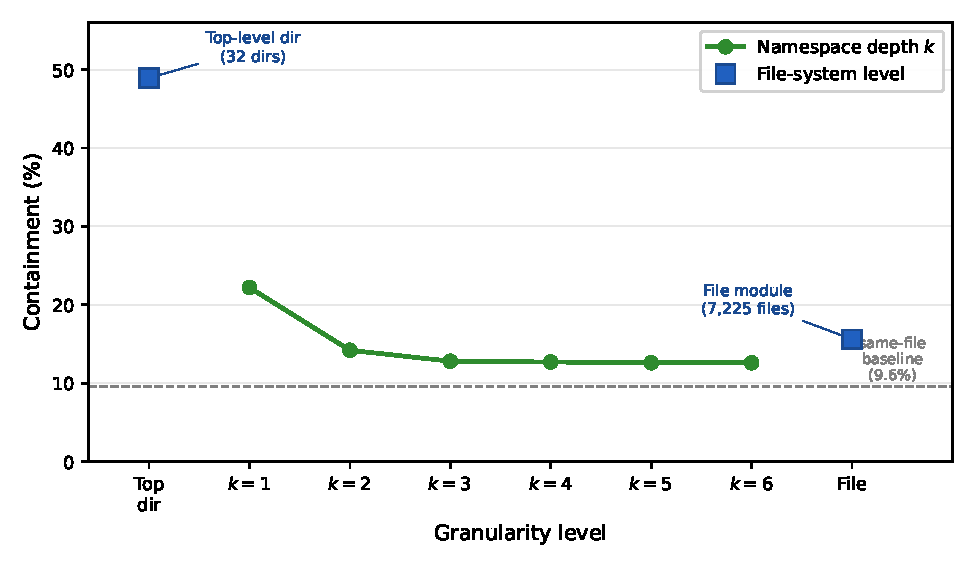
\includegraphics[width=0.82\textwidth]{analysis/containment_curve.pdf}
\caption{Containment decay curve. Red circles connected by the solid line show containment at namespace depth $k = 1, \ldots, 6$; blue squares mark file-system levels (top-level directory and file module). The gray dashed line marks the same-file baseline from Table~\ref{tab:thm-edge-breakdown} ($9.6\%$). Containment drops steeply from the top-level directory to depth~$1$ and saturates by depth~$3$.}
\label{fig:containment-curve}
\end{figure}

The decay exhibits three regimes.

\paragraph{Discipline-level containment (top-level directory, 48.9\%).} At the coarsest granularity---the $32$ top-level directories (\module{Algebra}, \module{CategoryTheory}, \module{Topology}, etc.)---nearly half of all declaration-level dependencies stay within the same directory. These discipline-level categories, inherited from centuries of mathematical practice, retain genuine organizational force: they capture the broadest fault lines of mathematical knowledge. Yet even here, more than half of all dependencies cross directory boundaries---confirming that no discipline is self-contained.

\paragraph{The steepest drop (top-level directory $\to$ depth~$1$, $48.9\% \to 22.2\%$).} The largest single decrease in containment occurs when we move from $32$ directories to $3{,}184$ depth-$1$ namespaces. This transition refines discipline-level groupings (such as the directory \module{Data}) into their internal constituents (\texttt{Nat}, \texttt{Int}, \texttt{List}, \texttt{Set}, \texttt{Finset}, etc.). The steep drop indicates that discipline-level classification exerts substantial constraint on dependencies, but once we enter the interior of a discipline, the namespace boundaries between \texttt{Nat} and \texttt{Int}---or between \texttt{Set} and \texttt{Finset}---carry far less force. Mathematics, at sub-discipline granularity, is deeply interconnected.

\paragraph{Rapid saturation (depth~$2$+, ${\sim}13\%$).} Beyond depth~$2$, containment barely decreases: from $14.2\%$ at depth~$2$ to $12.6\%$ at depth~$6$. Finer naming distinctions---separating \texttt{Nat.Prime} from \texttt{Nat}, or \texttt{CategoryTheory.Functor} from \texttt{CategoryTheory}---add almost no intra-namespace edges that were not already captured at depth~$2$. The cross-domain character of mathematical reasoning is fully exposed by the second level of the naming hierarchy.

\paragraph{File-level containment (15.6\%).} The file-module level ($7{,}225$ units) falls between namespace depth~$1$ ($3{,}184$) and depth~$2$ ($10{,}097$) in both granularity and containment. A source file aggregates declarations from potentially multiple sub-namespaces, giving it slightly more containment power than depth-$2$ namespaces of comparable count. But the difference is marginal: files, as organizational containers, offer no containment advantage beyond that of a mid-level namespace.

\subsection{Analysis}
\label{sec:ns-analysis}

The containment decay curve quantifies a central observation: \emph{the organizing power of human-imposed boundaries diminishes rapidly with granularity}. At the broadest scale, the disciplinary taxonomy that mathematicians have developed over centuries captures nearly half of the dependency structure. But this organizational force dissipates quickly once we move below the discipline level. By the time we reach depth-$2$ namespaces (${\sim}10{,}000$ groups), containment has fallen to $14\%$; further refinement adds almost nothing.

This pattern is consistent with the nature of formal mathematics. Logical dependencies are determined by the content of proofs, not by how humans choose to name and group results. A lemma about natural numbers may depend on ring theory, order theory, and decidability infrastructure; these dependencies pierce through any namespace boundary that a developer might draw. The namespace hierarchy provides a useful index for human navigation---one can browse ``all lemmas about primes'' by looking in \texttt{Nat.Prime}---but it does not delineate logical units. The containment decay curve makes this precise: the namespace is a cognitive aid whose structural content decays to a floor of ${\sim}13\%$ within two levels of refinement.

\begin{remark}
\label{rem:import-vs-decl-cross}
At the top-level directory level, $51.1\%$ of declaration-level dependencies cross directory boundaries. The module-level import graph, by contrast, shows only $37.1\%$ cross-directory edges (\S\ref{sec:cross-namespace}). The $14$-percentage-point gap arises because each import edge implicitly bundles many declaration-level dependencies: a single \texttt{import} from \module{Algebra} to \module{Data} may serve dozens of individual theorem citations that cross the same boundary. The import graph, as a human-authored summary of dependencies, is more ``inward-looking'' than the actual dependency structure it enables. This aligns with the import sparsity finding of \S\ref{sec:import_vs_declaration}: the import graph is a sparse cognitive proxy for the vastly denser declaration-level dependency network.
\end{remark}
